\chapterimage{Figures/aux_optics.png} % Chapter heading image
%PMC bench in the 10m AEI prototype copyright AEI
\chapter{Auxiliary Optics}
%\section{Auxiliary Optics}
\label{sec:Aux-optics}

\greencomment{Dave: I think this section could be *significantly*reduced in length.  The important things in this section are either related to finding components that will work at 1.5 and 2 um:
- high QE PDs
- EOMs and FIs
- wavefront sensors
or to managing stray light.\\
I don't think you need to go into great detail on Input Optics, Output Optics, Active Wavefront Sensing and Control.  They are all subsystems that need the things I mention above, so you can get away with saying "Many 3G interferometer subsystems (IO, OO, AWC) will require components working at 1.5 and 2 um..."}

\section{Introduction}
We use the term \emph{auxiliary optics} here for any optical subsystem not otherwise covered by a specific category (e.g. core optics or light sources). We further sub-categorize into these subsystems:
%However, since there are several major optical subsystems that fall into this category, it is useful to sub-categorize further.
The {\bf Input Optics} subsystem includes all optics between the light source and the input of the core interferometer, typically defined by the power recycling mirror. The {\bf Output Optics} subsystem includes all optics between the core interferometer output (typically defined by the signal recycling mirror) and the photo-detectors which detect the gravitational wave signal, with the exception of specific optical components used for the generation of squeezed light. The {\bf Active Wavefront Control} subsystem includes means for sensing and actively controlling the spatial properties of interferometer beams, with the typical goal of minimizing mode matching losses and contrast defects. The {\bf Stray Light Control} subsystem encompasses all design features which are intended to reduce the impact of stray light on the detector operations. Finally, the subcategory {\bf Other Auxiliary Optics} catches optical subsystems that fall neither into the other larger categories or the aforementioned auxiliary optics subcategories.

\section{Current State of the Art}
%In this section we briefly describe the current status of the key auxiliary optics subsystems in the foremost interferometric gravitational wave detectors. 
The {\bf Input optics} subsystem is responsible for delivering the laser light from the pre-stabilized laser (PSL) system to the core interferometer in the correct spatial mode, with the necessary phase modulation sidebands, as well as with the required frequency, intensity and alignment stability conditions. This subsystem therefore typically includes an electro-optic modulator (EOM) for producing the phase modulation, one or more suspended input mode cleaner (IMC) cavities, a power control system, and a input Faraday isolator (IFI) to protect the PSL from light reflected from the main interferometer. Detailed descriptions of the IO subsystems of aLIGO and AdVirgo can be found in Refs.~\cite{aLIGO_IO} and~\cite{IOchapter} respectively. 
%Electro-optic modulators (EOMs) are used to generate the phase modulation sidebands which are used for sensing the length and alignment of the core interferometer. Both aLIGO and AdVirgo use RTP as the electro-optic material in the EOMs due to its capability of handling the high throughout power~\cite{aLIGO_IO, adVirgo_IO}. The input Faraday isolator (IFI) is used to protect the PSL from reflected light from the interferometer, diverting it instead to another port where it can be detected and used for interferometer sensing and control. The high throughput power is one of the more challenging aspects of the IFI design, as it leads to thermal lensing and depolarization in the magneto-optic material (TGG in both aLIGO and AdVirgo). The input mode cleaner (IMC) is a suspended triangular cavity that serves (among others) the purpose of passively filtering out beam jitter from the PSL before injection into the main interferometer. 

\noindent
In the currently leading GW detectors, the {\bf Output optics} subsystem is responsible for filtering out higher-order spatial modes and unwanted control sidebands from the interferometer output light, and delivering the beam to the photodetectors where the GW signal measurement is made. The recent and planned squeezed light upgrades expand the role of this subsystem to include delivery of the squeezed beam to the main interferometer. This subsystem typically includes an output Faraday isolator, an output mode cleaner cavity (OMC), and high quantum efficiency photodiodes.

\noindent {\bf Active Wavefront Control} (AWC) is used in GW detectors to compensate for thermal effects caused by the absorption of light in the interferometer core optics. As the circulating light power goals increased from 1st to 2nd generation detectors, so too did the requirements for compensation of these thermal effects. The leading GW detectors have all implemented a range of active wavefront control methods including ring heaters, CO$_2$ laser heating, thermal radiation projection, and thermally deformable mirrors~\cite{aLIGO_AWC, AdVirgo_IO}. This subsystem is often conflated with the thermal compensation system (TCS), although TCS constitutes only a part of the AWC system. 

\noindent {\bf Stray Light Control}
mitigates the effects of light scattered out of the main beam and then scattered back into it as it can cause noise that can limit the sensitivity of the detector.
To address this problem, many precautions are taken in GW detectors to minimize the amount of light scattered out of the beam (by using high-quality smooth optical surfaces everywhere), and also to minimize the available paths for re-entry of scattered light into the main beam (by using baffles wherever possible). 

\noindent 
Examples for the category {\bf "Other Auxiliary Optics"} include 
%phase cameras (for separately detecting the spatial properties of the carrier and sidebands), 
auxiliary length sensing (ALS) systems for pre-stabilizing the arm cavities, and optical levers for local sensing of the alignment of optics.


%\paragraph{Introduction}
%In all the ground-based laser-interferometric gravitational wave detectors, the light which is injected into the main interferometer comes from high power lasers operating at 1064nm, with powers which could exceed 100 W (maximum 200W). Their frequency stability in the detection frequency band (10Hz-10kHz) is what you can find as the best in the world. Similarly, the relative intensity noise (RIN) of the laser beam is at the state of the art in laser power stabilization (2.10$^{-9}$/$\sqrt(Hz)$). Their spatial eigenmode is very close to an ideal Gaussian mode. In a first paragraph, we will give an overview of the function carried out by the Input optics.
%
%\paragraph {Overview}
%
%The Input Optics is the interface between the laser system and the Interferometer. It is also part of the Pre-stabilized laser. The whole system delivers a beam at the interferometer input port with the required power, geometrical shape, frequency and angular stability. An Electro Optic Modulation (EOM) system is providing the RF modulations needed for control and sensing purposes. The Input Mode Cleaner (IMC) cavity geometrically cleans the beam and reduces its amplitude and lateral fluctuation. The resonant IMC in conjunction with a reference cavity (RFC) are used to stabilize the laser frequency.
%After the IMC some photodetectors provide the signal for intensity stabilization of the laser. An in-vacuum Faraday isolator prevents the light reflected by the interferometer goes back to the laser system and allows a simple extraction of this reflected beam. Finally, a mode matching telescope is used to properly match the beam on the Interferometer.
%
%\paragraph {Wavelength and power handling}
%In the first and second generation of GW detectors based on laser interferometers, the working wavelength is 1064nm which is produced by Nd:YAG solid state lasers. The power of the laser source in the first generation was of the order of a few tens of Watts which became a few hundred of Watts for the second generation. Up to now the detectors have been operated at a maximum of 50Watts injected in the interferometer but the plan is to reach 125Watts in the later developments of this generation. Due to the high power densities in the optical components such as the EOM system and the Faraday isolator, those devices has been specially developed for the Gravitational Wave detectors. 
%
%\paragraph {Electro optic modulation system}
%State of the art of the EOMs currently used will be given here.
%
%\paragraph {Faraday isolators}
%State of the art of the FIs currently used will be given here.
%
%\paragraph {Input mode cleaner}
%State of the art of the IMC cavities currently used will be given here.
%Why Geo uses 2 IMCs?
%
%\begin{table}[htp]
%\begin{tabular}{@{}l c c c c c@{}}
%Parameter & LIGO & Virgo & GEO & &Kagra\\
%       &  &   &  IMC1  & IMC2 &  \\
%\hline
%Optical cavity length & 32.945 m & 286.845 m & 8 m & 8.1 m & 53.3m (TBC)\\
%Free spectral range & 9,099,786 Hz & 1,045,137 Hz & 37.48 MHz & 37.12 MHz &\\
%Radius of curvature of MC2 & 27.27 m & 185.1 m& & &\\
%Flat mirror transmissivities & 6000 ppm & 2880 ppm & & & 6000 ppm \\
%MC2 transmissivity & 5 ppm & 2.2 ppm & & &< 200ppm\\
%Cavity Pole frequency & 8.72 kHz & 520 Hz & & & \\
%\hline
%\end{tabular}
%\label{IMC cavities main parameters}
%\end{table}
%
%\paragraph{Mode matching telescope}
%MMT will be described here and some references will be given.
%
%\paragraph {Performances and issues}
%In this paragraph we will describe the performances obtained (firstly underlining that GWs have been detected both with LIGO and Virgo). Then, we can write a few sentences on the beam jitter which represents one of the most annoying technical noises we can find at the level of the IO in the current generation. There are some possible mitigations (such as increasing beam jitter reduction in vacuum as underlined by Matt and proposed in LIGO (See Jitter Attenuation Cavity \url{https://dcc.ligo.org/LIGO-T1600595}))
%
%\subsubsection{Output optics}
%The output optics subsystem of interferometric GW detectors typically refers to all optics in the detection chain after the signal recycling mirror. In the advanced generation of detectors, this includes the beam steering optics, output Faraday isolator, output mode cleaner, and photodetectors. For squeezing enhanced detectors, the output optics includes all optics between the squeezing source and the main interferometer, as well as probably alignment sensing and control, a squeezing phase sensing and control scheme, and mode matching optics.
%In A+, the near term upgrade to Advanced LIGO, this will also include the 300\,m filter cavity which is used to provide frequency dependent squeezing for sensitivity enhancement at all frequencies in the detection band. 
%
%\paragraph {Output mode cleaner}
%Advanced LIGO employ suspended in-vacuum 4-mirror output mode cleaner cavities (OMCs). Advanced Virgo use 2 monolithic OMC cavities in series. 
%These cavities are used for two primary purposes: to clean the spatial mode of the interferometer output beam (rejecting higher-order spatial modes which add shot noise but no signal), and to remove the rf sidebands from the light which reaches the photodetectors which are used to read out the GW signal. OMCs are necessary for the DC readout scheme which has been in use since GEO600, enhanced LIGO and Virgo+ (fact check please)~\cite{dcreadout}. 
%The output mode cleaner cavity should be designed such that the sidebands HG$_{00}$ mode and all higher-order modes are not co-resonant with the carrier frequency HG$_{00}$ mode. Scattered light in the OMC is also a serious concern. 
%Add some more detail here on the aLIGO and AdVirgo OMCs. Anything for A+ or 3G OMCs?
%
%\paragraph{Photodetectors}
%The photodetectors which are currently used for the GW signal detection are all InGaAs detectors, which have been screened for high quantum efficiency at 1064\,nm. Most of the current R\&D into high-quantum efficiency is aimed at longer wavelengths. Some details here perhaps on where the aLIGO and AdVirgo PDs were sourced from. Who is working on high-QE PDs at 1550\,nm.
%
%\paragraph{Balanced homodyne detection}
%The LSC currently has a specific subgroup which has been tasked with developing the necessary designs and technology for implementing balanced homodyne detection (BHD) in the A+ interferometers. Balanced homodyne detection requires that the output light from the interferometer is interfered against a stable reference field. Adjusting the relative phase of the two fields allows to adjust the readout quadrature of the GW signal. In the currently used DC readout scheme carrier light from within the interferometer is used as the reference field, by slightly detuning the differential arm length (DARM) degree of freedom. In this scheme, however, the phase of the reference field cannot be adjusted against the GW signal field. The LSC BHD R\&D is coordinated through the LSC wiki page here: \url{https://wiki.ligo.org/AIC/BHD_A_plus}. Stefan Hild from the University of Glasgow is leading this effort. Any knowledge of efforts at AdVirgo to include BHD?
%
%\paragraph{Filter cavities}
%Filter cavities have been a topic of research within the GW community since they were demonstrated to effectively rotate the squeezing angle (or quadrature) of squeezed light reflected from the cavity in the frequency band around resonance~\cite{chelkowski}. Initial demonstrations were performed for squeezing at Fourier frequencies in the rf band, but in recent years frequency dependent squeezing with filter cavities was demonstrated in the audio frequency band~\cite{MITfiltercav}. Frequency dependent squeezing becomes necessary for GW detectors as the detectors become increasingly limited by quantum noise, both at the high frequency end of the measurement band (shot noise) and the low frequency end (quantum radiation pressure noise). Frequency independent squeezing can only improve one of these quantum noise effects, while exacerbating the other. The filter cavity must have a linewidth which is close to that of the core interferometer for GW signal sidebands. In the case of Advanced LIGO, this value is roughly 100\,Hz (fact check please). To make a filter cavity with such small linewidth, the cavity must either be extremely long, or extremely high finesse. In the high-finesse case, optical losses at the mirror surfaces become increasingly significant, leading to a degradation in the squeezing depth. It is an active topic of research in the community to determine the optimal filter cavity parameters with regards to length and finesse, although designs for A+ are being consolidated currently. Something about who is working on filter cavities here... 
%
%\paragraph{Low-loss Faraday isolator}
%The output Faraday isolator (OFI) is currently used to reject backscattered light from the photodetectors and OMC from re-entering the interferometer. Optical losses in the OFI currently do not have a severe impact on the detector sensitivity, they simply degrade the signal by reducing the total amount of light reaching the photodetectors. In principle this can be compensated by simply using a larger DARM offset.
%With the addition of squeezed light enhancement however, optical losses in the OFI becomes much more critical. In a squeezing enhanced interferometer, the OFI also serves a second purpose as the injection port for the squeezed light. The squeezed light passes through the OFI twice before reaching the photodetectors. Optical losses in the squeezing path reduce the effective squeezing severely, and if bad enough will actually make the quantum noise limited sensitivity worse than with no squeezing at all~\cite{dwyer}. Low-loss Faraday isolators is therefore seen throughout the community as a critical R\&D topic for output optics in the drive towards 3G sensitivities.
%Faraday isolators exhibiting single pass losses $\leq$ 1\% have been installed on the Advanced Virgo detector in February 2018 (add reference).
%
%\subsubsection{Active wavefront control}
%Active wavefront control (AWC) is a term which has been coined to cover the sensing and control of all beam mismatches and imperfections in the optical chain which are of a higher spatial frequency than simple misalignment. At the first order, this corresponds to spherical mode mismatches between the various beam and cavity eigenmodes. AWC also in principle includes higher-order wavefront distortions such as astigmatism, coma, trefoil and so on. In many cases, the spatial mode in the interferometer cavities is laser power-dependent, due to absorption in the substrates and coatings of the optics. In other cases mode mismatches result simply from imperfect placement of optics, or from fixed deviations of the optics from design specifications. Several different AWC technologies have been developed in order to manage the many different kinds of mode mismatches in the interferometers. We will give a brief description of these here.
%
%\paragraph{Core optics thermal compensation}
%\begin{itemize}
%\item Ring heaters
%\item CO$_{2}$ laser and compensation plates.
%\item Projected heaters (CHROCC), SR3 heater at aLIGO etc.
%\item anything else?
%\end{itemize}
%\paragraph{Input mode matching}
%\begin{itemize}
%\item UF/Syracuse thermal lens
%\item backside heated mirror
%\item anything else?
%\end{itemize}
%
%\paragraph{Output mode matching}
%\begin{itemize}
%\item UF/Syracuse thermal lens
%\item backside heated mirror
%\item anything else?
%\item this is extra critical because of squeezing, losses etc.
%\end{itemize}
%\paragraph{Mismatch sensing}
%\begin{itemize}
%\item Phase camera
%\item Hartman sensor
%\item Bullseye sensor
%\item Mode converter and QPD
%\item Beam size jitter sensing
%\end{itemize}
%\subsubsection{Stray light control}
%\paragraph{Baffles}
%Something about what was done with baffling at aLIGO and AdVirgo. What worked well and what did not? What has already been earmarked for upgrades?
%
%\paragraph{Optics}
%What did we learn from aLIGO and AdVirgo about scattering from optics?
%
%\subsubsection{Other auxiliary optics}
%
%\paragraph{Optical levers}
%\paragraph{Alignment sensing schemes}
%
\section{Requirements, challenges and current/planned R\&D}
\subsection{Input optics}
 Future 3G GW detectors will require different input optics than the current second-generation detectors. The way in which the input optics will differ depends heavily on some of the design decisions for 3G detectors, many of which have not yet been made. Most critical for the input optics will be the choice of laser wavelength; the EOM and IFI rely on unusual electro- and magneto-optic materials that may have significantly different characteristics at longer wavelengths. Choosing suitable materials is not expected to pose a great challenge if the wavelength is changed to 1550\,nm, but 2+$\mu$m will probably require considerable effort. The high power transmitted through these optics makes low absorption critical (due to the resulting thermal lensing and depolarization effects), thus further narrowing the choise of suitable material. At 2$\mu$m Faraday isolators already exist~\cite{EOTFI}, but a high power vacuum compatible one must be developed as it is not commercially available. Iron garnets should be considered as potential candidates for the magneto-optic material for 2+$\mu$m light, also
%. It could be Yttrium Iron Garnet (YIG) or bismuth-substituted iron garnet. Those materials 
having the advantage that the Faraday rotation effect is an order of magnitude larger than that of TGG in the near infrared range, allowing a reduction in magnet size and the overall footprint and weight of the device.
The IMC design is not expected to fundamentally change beyond the 2nd generation.  However, AdVirgo and aLIGO have both seen that noise contributions have been limited by beam jitte~\cite{aLIGOjitter,adVirgojitter} so that increasing the IMC finesse or adding a second IMC in series with the first could be a way to further suppress the beam jitter. Another possibility is to reduce the beam jitter at the source, either passively or with high bandwidth control loops.  

In addition to upgrades and modifications of existing IO components, several new components are also being researched. High bandwidth electro-optic beam deflectors could be used as actuators for beam jitter suppression loops and for providing alignment sidebands for an alternative method of alignment sensing in both the IMC and in the core interferometer~\cite{RFJASC}. The use of higher-order modes for coating thermal noise reduction is still under consideration for 3G interferometers~\cite{LGmodes}. If this technology is pursued further, the higher-order mode conversion/preparation path is likely to be incorporated into the IO remit. 
%Although significant advances have been made in this direction in the last decade~\cite{LGmodes1,LGmodes2}, further R\&D will be necessary to bring the technology to the required readiness level for 3G detectors. 
The use of complex modulation~\cite{complexmod} and parallel modulation~\cite{kagraMZI} are also under investigation for reducing sidebands-of-sidebands effects that may limit interferometer sensing and control performance.

\subsection{Output optics}
\magentacomment{hal: include need to develop robust length and angular DoFs control schemes for detuned filter cavities and finesse control to control pole frequency}
With all 3G concepts assuming significant enhancement from the use of squeezed light, the critical feature for the 3G output optics will be ultra-low optical losses~\cite{squeeze_lossbudget}. OFIs with reduced optical losses are being developed~\cite{EGOLLFI,UFLLFI}, for use in the advanced GW detectors. Figure~\ref{fig:AdVLLFI} shows the low-loss OFI which has recently been installed in Advanced Virgo. OMCs must also be designed for high throughput, and photodetectors must have high quantum efficiency (QE). High-QE photodetectors at longer wavelengths has been identified as a crucial R\&D task; one which may be especially onerous for 2+$\mu$m light. Frequency dependent squeezing will also require the inclusion of a filter cavity (FC) in the path between the squeezed light source and the OFI. 300\,m long FCs are planned for the near-term upgrades to aLIGO and AdV, following on from R\&D performed at MIT~\cite{MITFC} and in Japan\cite{TAMA_FDS2016}. Alternative readout schemes such as balanced homodyne detection (BHD - another project planned for inclusion in A+) will require a redesign of the output optics chain~\cite{BHD}.

\begin{figure}[htb]
\centering
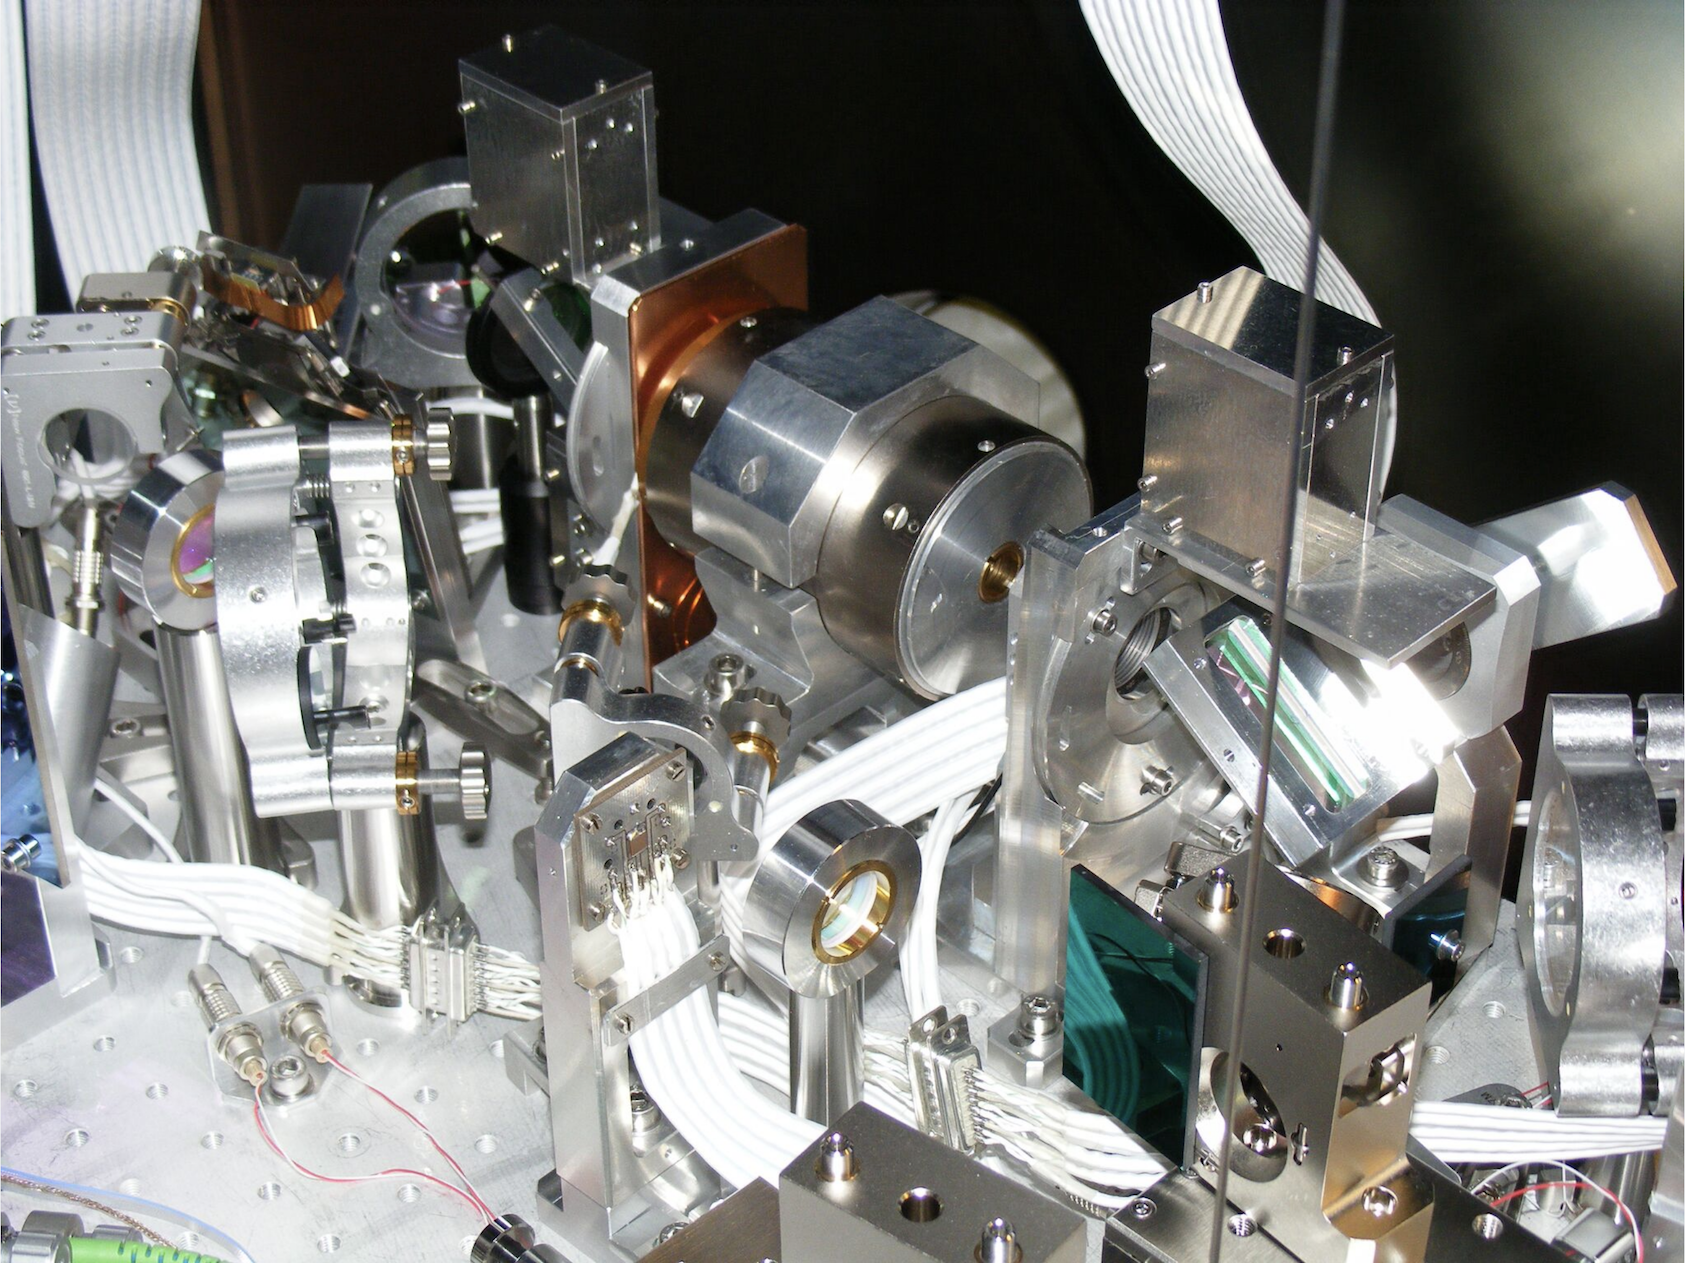
\includegraphics[width=0.6\textwidth]{Figures/LLFI.png}
\caption{The low-loss OFI upgrade to Advanced Virgo, recently installed ahead of the third observing run of the advanced detector era.\label{fig:AdVLLFI}}
\end{figure}

%\begin{itemize}
%\item BHD
%\item filter cavities
%\item high QE PDs at new wavelengths
%\item high throughout OFIs
%\item high throughput OMCs
%\end{itemize}

\subsection{Active wavefront control}
In 1st and 2nd generation detectors, active wavefront control (AWC) has often been implemented in something of an \emph{ad hoc} way. In no cases has a feedback loop been used to maintain mode matching in a detector during normal operations. This is partly due to the low bandwidth of the typical actuators, but also due to the limitations in the AWC sensors available. As a result, AWC is typically employed in a set-and-forget manner, which requires frequent manual retuning as the circulating power in the interferometer changes. 3G detectors will likely require higher performance from the AWC subsystem for several reasons: higher circulating powers, larger thermal gradients under cryogenic operation, larger beams with flatter wavefronts, and stricter requirements on optical losses. An LSC white paper on AWC has been written to track the LSC R\&D in this direction~\cite{aLIGO_AWC}, and similar work is planned for AdV+. AWC R\&D for 3G detectors is expected to focus on new sensors (RF bullseye wavefront sensors~\cite{bullseye}, improved Hartmann wavefront sensors~\cite{HWS}, phase cameras~\cite{phasecam}), as well as actuators (converting existing actuators for new optic materials, and developing new actuators). 
 
%\begin{itemize}
%\item mismatch sensors (HWS, bullseye, etc.)
%\item mismatch actuators
%\item needed in more locations, esp. output chain.
%\end{itemize}

\subsection{Stray light control}
Although it is often difficult to diagnose directly, stray light was expected to be  limiting the sensitivity of both aLIGO and AdVirgo during O2. As such, improvements must clearly be made in order to reach 3G sensitivities with any methods other than extending the baseline length. Continued R\&D into mirror polishing and coating techniques to give improved surface roughness will go some way to reducing stray light contributions, as will the development of better baffling materials with lower reflectivities. One concern is that if the laser wavelength is changed to 2+$\mu$m, finding good absorbers for baffle materials may become more difficult. 

%\begin{itemize}
%\item baffle material for longer wavelengths?
%\item more baffles?
%\item what else to say here? coating/polishing/cleanliness development?
%\end{itemize}

\subsection{Other auxiliary optics}
AdVirgo, aLIGO and Kagra all either use (or provision for) an auxiliary length sensing system in order to make the interferometer locking process deterministic. Since the optical layout of 3G detectors is not expected to reduce in complexity, it seems natural that similar systems will be required in the future. Optical levers are  omnipresent in 2G detectors, and provide important information about angular motion of the optics. Increased sensitivity in these local sensors may be beneficial for 3G detectors with increased baselines and sensitivity goals, and accordingly R\&D is ongoing towards that end. Suspension point interferometry (SPI)~\cite{SPI} may be a useful technique for reducing low frequency control noise in 3G detectors, and will require an additional auxiliary optical subsystem. SPI is currently being used at the AEI 10\,m prototype interferometer.   

%\tcr{include figure here with the table of R\&D}
\subsection{Survey of current auxiliary optics R\&D }
A survey was conducted throughout research groups who are known to be working on, or have previously worked on auxiliary optics topics. A living document (accessible at \url{https://goo.gl/W9mrCj}) shows the current status of the worldwide auxiliary optics R\&D, as informed by this survey. 

% \magentacomment{hal: Include pointer to a living document instead of static table? Suggested by GWIC 3G committee}

% \begin{figure}[htb]
% \centering
% 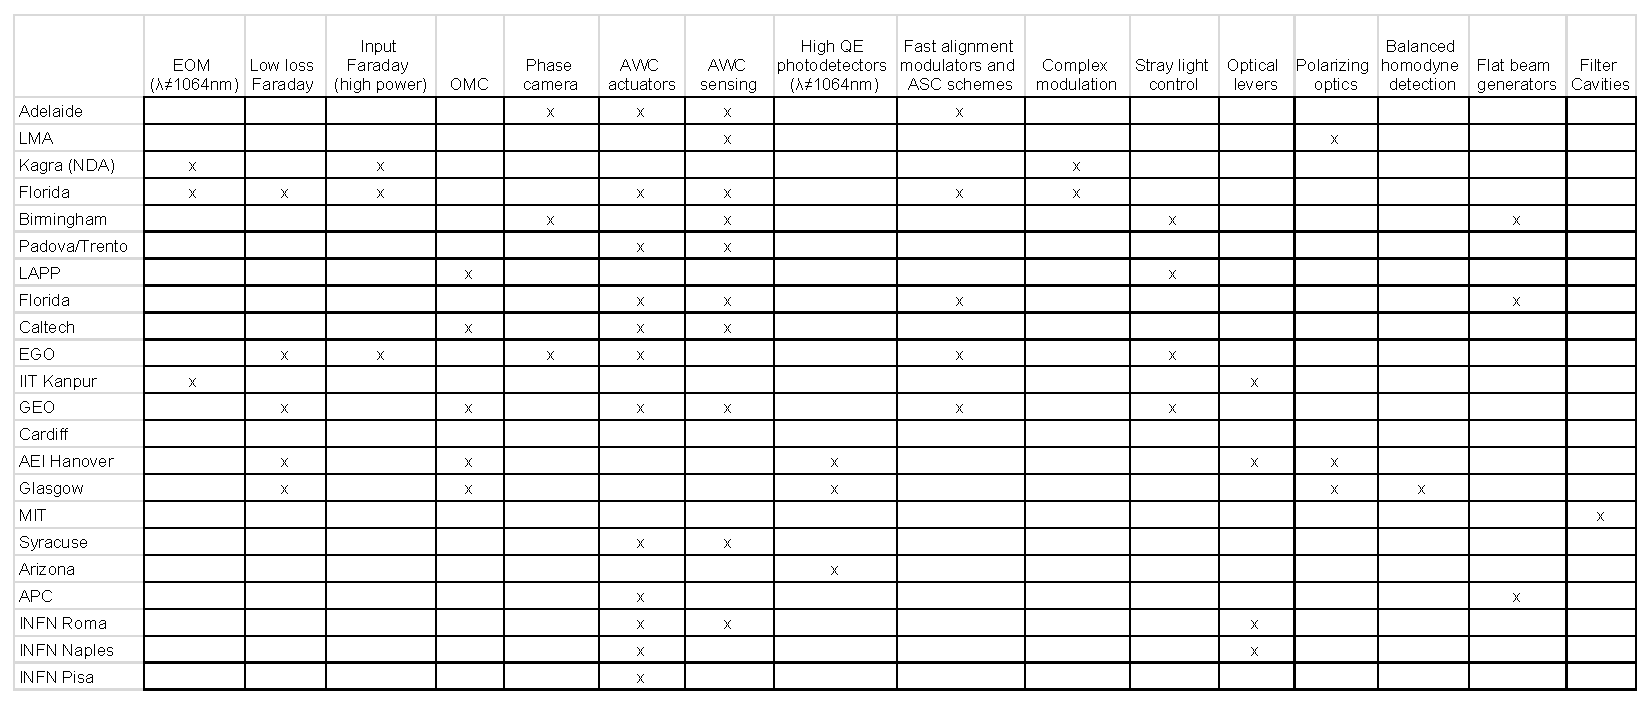
\includegraphics[width=\textwidth]{Figures/AUXopticssurvey.pdf}
% \caption{The current status of global gravitational wave detector auxiliary optics R\&D, based on the responses to an email survey and the knowledge of subcommittee members.\label{fig:auxopticssurvey}}
% \end{figure}
%
%The remainder of this section is subdivided into a discussion of the requirements for each auxiliary optics subcategory in the context of laser wavelengths between 1 and 1.55\,$\mu$m and 1.55\,$\mu$m and above. Where there is expected to be no major difference between the R\&D required for both wavelength ranges, the R\&D will be described in the section for the shorter wavelength range only. 
%
%\subsubsection{1-1.55\,$\mu$m laser wavelength R\&D requirements}
%\paragraph{Input optics}
%In that wavelength range, we do not expect particular issues with respect to the 2G. The main issue might concern scattered light management and beam jitter mitigation.
%We mostly rely the developments which have been made for the first and second generation of GW detectors at 1.064 $\mu$m. For 1.55$\mu$m, there will be for sure the need of R\&D on wavelength dependent optical devices such as the Faraday isolator especially if we want to work at very high power at 1.55$\mu$m. Some R\&D activities are already planned in several groups (IAP, UF and EGO) so we do not expect major issues on that point.
%Below we just list the most important sub-parts of the IO.
%\begin{itemize}
%\item	High power Faraday isolator for 1 and 1.55 um R\&D on-going.
%\item	EOMs. Seems to be under control but might be needed to think about RAM noise.
%\item	Complex modulation - can be used to minimize am (better control of locking point offsets). R\&D ongoing.
%\item	Fast alignment actuators. Alignment sensing and/or control. R\&D ongoing.
%\item	Flat beam generators (LG modes etc.). Not much active research recently.
%\item	Input mode cleaner and frequency stabilization scheme (not R\&D more related to design choices). 
%\end{itemize}
%\paragraph{Output optics}
%The main point will consist in mitigating the scattered light which is harmful for the Interferometer sensitivities in the second generation of GW detector.
%R\&D activity on OMC could be useful?
%For what concerns the development of low-loss Faraday isolator for the squeezed light injection at 1$\mu$m, the situation seems well under control. A few groups are working on that topic (UF,AEI and EGO). Some good results have been obtained recently with the demonstration of sub percent loss Faraday isolators (see for example refLLFI). We can reasonably expect to get below 0.5\% for a single pass. If the losses have to be lower some particular effort will have to be devoted to that topic.\\ 
%Filter cavity
%
%refLLFI E. Genin and G. Pillant, Development of Low loss Faraday isolators at EGO, Presentation at LVC Sonoma meeting, March 2018, \url{https://dcc.ligo.org/DocDB/0150/G1800468/001/LowlossFIupdate_20032018_v2.pdf}
%
%\paragraph{Active wavefront control}
%At 1um we can base the TCS system on what has been used in the second generation GW detectors.
%At 1.55$\mu$m, it could be required to change the actuation techniques if we change the test mass material. 
%In general we expect that the requirements on mode matching and contrast defect become significantly more stringent for upgrades to the Advanced detectors, and for the 3G detectors. This is primarily because of the expected addition of squeezed light enhanced to the detectors. Mode mismatches in the core interferometer and the signal extraction chain can cause at best a reduction in the benefit of squeezing at certain frequencies (i.e. in the case of mode mismatch to a filter cavity), and at worst an effective optical loss 
%
%\paragraph{Stray light mitigation}
%The light absorption from the baffles is very dependent on the wavelength. So it is likely that what will work at 1um but not at 1.55 $\mu$m. R\&D will be required to find new materials suitable for 1.55$\mu$m.  
%
%\paragraph{Other auxiliary optics}
%{\bf Optical levers}
%Increasing the length of the arm cavities can represent a problem from the optical levers point of view. A preliminary study should be done in order to understand the requirements on the suspended optics residual motion tolerated to be able to lock the arm cavities (40 km is quite long!).
%
%{\bf Alignment sensing schemes}
%
%{\bf Polarization optics}
%In the case that a Sagnac-type interferometer is to be used for 3G detectors, one option will be a polarization based Sagnac
%
%\subsubsection{1.55+\,$\mu$m laser wavelength R\&D requirements}
%Above 1.55 $\mu$m and especially if we go to 2 or 2.1 $\mu$m things are new and it is sure exploratory activities will be required. Consider that now most in the laboratories involved in the business are equipped with optics laser sources and detectors for 1 $\mu$m wavelength. Going to 2 $\mu$m will require a huge funding effort form the agencies.\\
%
%\paragraph{Input optics}
%
%The most critical components remain the one which are wavelength dependent such as the Faraday isolator in particular.  Some R\&D activities are already planned in several groups (IAP, UF and EGO) to develop a high power vacuum compatible Faraday isolator for 2 $\mu$m.
%At 2$\mu$m, Faraday isolators already exist (refEoT) but a high power vacuum compatible one will have to be developed since it cannot be found on the market. In that case, iron garnets should be considered as potential candidates. It could be Yttrium Iron Garnet (YIG) or bismuth-substituted iron garnet. Those materials have the advantage that the Faraday rotation effect is one order of magnitude larger than that of TGG in the near infrared region. This could help reducing the magnet size and the overall weight of the device.\\
%
%refEoT EoT Makros series, \url{https://www.eotech.com/cart/3/faraday-rotators/makros-series-1900-2100nm-high-power-faraday-rotators}\\
%
%Regarding the Electro optic modulation system, according to what we know Rubidium Titanyl Phosphate could be kept as EO crystal since it is also transparent on a wide wavelength range (0.5$\mu$m to 3.5$\mu$m) but some tests will have to be made in order to evaluate the absorption of this crystal at 2 $\mu$m which could represent an issue if high.
%
%\paragraph{Output optics}
%\paragraph{Active wavefront control}
%\paragraph{Stray light mitigation}
%\paragraph{Other auxiliary optics}
%
% \subsubsection{3G initial}
% \subsubsection{future}
\section{Pathways, required facilities, collaborations and mechanisms}
\subsection{Pathways and required facilities}
Many of the auxiliary optics subsystems R\&D, such as for example materials investigations for EOMs and FIs, can be performed in small laboratories. 
Some of the larger subsystems such as filter cavities, on the other hand, require larger integrated facilities for testing. In many cases the 3G auxiliary optics technologies will also be included in upgrades to the 2nd generation detectors such as A+, AdV+ and Kagra. Simply by virtue of being \emph{auxiliary}, modular upgrades in many of these technologies are possible. Modular upgrades are probably not feasible in the case of a change in the main laser wavelength, however. Such a change for 3G detectors will necessitate a broader range of auxiliary optics R\&D, which might benefit from a more complete demonstration on prototype detectors such as the Caltech 40m prototype, or the Glasgow and AEI 10m prototype detectors. The GEO600 detector has frequently proved an excellent testing ground for new GW detector technologies, and so could also have an important role to play in developing 3G auxiliary optics technology. The LIGO Voyager plans already center around a change in wavelength, and so this will also be an important proving ground for 3G non-1064\,nm auxiliary optics.
%2G upgrades such as A+, AdV+ and longer term, LIGO Voyager or similar, will also likely be excellent testing grounds for new auxiliary optics subsystems prior to inclusion in 3G detectors. 

\subsection{Collaborations between groups working on the different AO topics identified}
%\begin{itemize}
\subsubsection{\bf Input optics} The groups working on IO for 2nd generation upgrades and beyond are primarily those groups who have worked on providing input optics for aLIGO, AdVirgo, GEO and Kagra in the past. In the LSC-Virgo collaboration information is shared on progress in development of future input optics mostly through the auxiliary optics working group, with talks and posters at collaboration meetings. This method of collaboration seems to be sufficient for now. If the community steers towards a change in wavelength, however, additional information exchange mechanisms may be required in order to accelerate the development of suitable input optics components.

\subsubsection{\bf Output optics} The key features for the output optics of 2nd generation upgrades and beyond are minimizing optical losses, while adding further subsystems such as filter cavities and balanced homodyne detection paths. 
%The authors are not aware of specific collaborations beyond those internal to the LSC, Virgo and Kagra collaborations. Presumably information will be exchanged at collaboration meetings, GWADW, and Amaldi meetings in the usual way. 
Low-loss output Faraday isolators are slated for inclusion in near-term 2G detector upgrades, so it might be useful for the 5 groups identified to be working on this to have a dedicated workshop to discuss progress and plans in the near future. 

\subsubsection{\bf Active wavefront control} This subsystem was identified by the authors as being one which could benefit from increased global collaboration. Due to the \emph{ad hoc} nature of this subsystem's prior development, many groups have followed individual paths towards distinct but often similar solutions. We suggest that the formation of an active wavefront control subgroup will help to focus the efforts of the community towards a common goal of a suitable wavefront sensing and control strategy for future GW detectors. 

\subsubsection{\bf Stray light control} This subsystem could benefit from the collaboration between groups worldwide if the laser wavelength chosen is the same for all of the next generation GW detectors. If different choices are made, each project should organize R\&D activities on their own. From the stray light control perspective at least therefore, significant savings in time and money could be made by choosing common wavelengths between 3G detectors. 

\subsubsection{\bf Other auxiliary optics} Unless required by groups working on auxiliary optics topics outside the scope of the aforementioned, specific collaboration mechanisms are not seen as a priority at this time. 

%\end{itemize}
\subsection{Collaborations between AO and other subsystems}
%\begin{itemize}
\paragraph{\bf Light sources} As previously mentioned, many of the auxiliary optics subsystems will be strongly impacted by the choice of laser wavelength going forward. Beyond this, the input optics has a direct interface with the light source, and so information exchange between groups performing R\&D on these two areas will be critical.
\subsubsection{\bf Quantum noise} The output optics subsystem will be closely linked to the quantum noise working groups for the forseeable future, with the now expected inclusion of squeezing in all future detectors. Close collaboration between these groups will therefore be beneficial.
%\end{itemize}

%\item specific mention of the AWC effort benefiting form some global coordination.
%\end{itemize}
%\subsubsection{Suggested mechanisms}
%%
%How do we get these things together? Maybe an AWC workshop some time?
%
%\subsection{Impact/relation to 2G and upgrades}
%
%This is kind of already covered in the previous sections, where some 3G-ish AO will be tested on 2.5G detectors, or is already being planned for 2G detectors (e.g. LLFIs in aLIGO for O4 and LLFI in AdVirgo for O3). Maybe just take this out...
%%\paragraph{Input optics}
%%
%%
%%\paragraph{Output optics}
%%Filter cavities are being planned for installation at the Advanced LIGO and Advanced Virgo detectors as part of the A+ upgrade for Ligo and AdV+ upgrade for Virgo. We expect that some type of frequency dependent squeezing enhancement will be included in all 3G detectors, so the inclusion in the 2nd generation upgrades is of course beneficial in terms of preparatory R\&D.
%%
%%\paragraph{Active wavefront control}
%%\paragraph{Stray light mitigation}
%%\paragraph{Other auxiliary optics}
%%%\section{}
%%%\subsection{}
%%

%\begin{thebibliography}{10}
%\newcommand{\enquote}[1]{``#1''}

%\bibitem{aLIGO_IO} C.L. Mueller \emph{et al}, \emph{The advanced LIGO input optics}, Rev. of Sci. Instr. {\bf 87}, 014502 (2016).

%\bibitem{IOchapter} E. Genin, G. Mueller, \emph{Input optics}, Book chapter, in editorial process (2018).

%\bibitem{aLIGO_AWC} A.~F. Brooks, R.~X. Adhikari, S. Ballmer, L. Barsotti, P. Fulda, A. Perreca, \emph{Active wavefront control roadmap}, LIGO Document LIGO-T1500188-v5 (2015).

%\bibitem{AdVirgo_IO} The Virgo collaboration, \emph{Advanced Virgo technical design report}, Virgo internal document VIR-0128A-12 (2012).

%\bibitem{EOTFI} \url{https://www.eotech.com/cart/37/free-space-optical-isolators}.

%\bibitem{adVirgojitter} B. Canuel, E. Genin, M. Mantovani, J. Marque, P. Ruggi and M. Tacca, \emph{Sub-nanoradian beam pointing monitoring and stabilization system for controlling input beam jitter in gravitational wave interferometers}, Appl. Opt. {\bf 53}, 2906-2916 (2014).

%\bibitem{aLIGOjitter} D.~V. Martynov \emph{et al}, \emph{Sensitivity of the Advanced LIGO detectors at the beginning of gravitational wave astronomy}, Phys. Rev. D. {\bf 93} 112004 (2016).

%\bibitem{RFJASC} P. Fulda, D. Voss, C. Mueller, L.~F. Ortega, G. Ciani, G. Mueller, D.~B. Tanner, \emph{Alignment sensing for optical cavities using RF jitter modulation}, Appl. Opt. {\bf 56} 3879-3888 (2017).

%\bibitem{LGmodes} A. Noack, C. Bogan, and B. Willke, \emph{Higher-order Laguerre–Gauss modes in (non-) planar four-mirror cavities for future gravitational wave detectors} , Opt. Lett. {\bf 42} 751-754 (2017).

%\bibitem{complexmod} D.~B. Tanner, T. Uehara, V. Quetschke, G. Mueller, H. Chia and G. Ciani, \emph{Complex Modulation}, LIGO Document LIGO-T170470-v41 (2017). 

%\bibitem{kagraMZI} KAGRA Main Interferometer Working Group, \emph{KAGRA Main Interferometer Design Document}, Kagra Document T1200913 (2012).
 
 %\bibitem{squeeze_lossbudget} E. Oelker, L. Barsotti, S. Dwyer, D. Sigg and N. Mavalvala, \emph{Squeezed light for advanced gravitational wave detectors and beyond}, Opt. Express {\bf 22} 21106-21121 (2014). 
 
 %\bibitem{EGOLLFI} E. Genin, G. Pillant,  M. Mantovani, M. Gosselin, C. De Rossi, J. Casanueva, L. Pinard, and C. Michel, \emph{Vacuum compatible low losses Faraday isolator for efficient squeezed light injection in Laser interferometer based Gravitational wave detectors}, Appl. Opt., {\bf 34} 34 (2018).
 
 %\bibitem{UFLLFI} R. Goetz, \emph{A Low Loss Faraday Isolator for Squeezing Injection in Advanced LIGO, and Radio-Frequency Amplitude Modulation}, PhD thesis (2017).

%\bibitem{MITFC} E. Oelker, T. Isogai, J. Miller, M. Tse, L. Barsotti, N. Mavalvala, and M. Evans, \emph{Audio-Band Frequency-Dependent Squeezing for Gravitational-Wave Detectors}, Phys. Rev. Lett. {\bf 116} 041102 (2016).

%\bibitem{BHD} P. Fritschel, M. Evans, and V. Frolov, \emph{Balanced homodyne readout for quantum limited gravitational wave detectors}, Opt. Express {\bf 22} 4224-4234 (2014).

%\bibitem{bullseye} G. Mueller, Q. Shu, R.~X. Adhikari, D.~B. Tanner, D. Reitze, D. Sigg, N. Mavalvala and J. Camp, \emph{Determination and optimization of mode matching into optical cavities by heterodyne detection}, Opt. Lett. {\bf 25} 266-268 (2000).

%\bibitem{HWS} P. Veitch, A.~F. Brooks, W. Kim, C. Blair, H. Cao, G. Grabeel, T. Hardwick, M. Heintze, A. Heponstall, C. Ingram, J. Munch, D. Ottaway, and T. Vo, \emph{Hartmann Wavefront Sensors for Advanced LIGO}, Proc. CLEO SI SW3M (2018).

%\bibitem{phasecam}  L. van der Schaaf, K. Agatsuma, M. van Beuzekom, M. Gebyehu and J. van den Brand, 2016 J. Phys.: Conf. Ser. {\bf 718} 072008 (2016).

%\end{thebibliography}